\documentclass{standalone}

\usepackage{siunitx}
\usepackage{pgfplots}
\usepackage{pgfplotstable}

\begin{document}

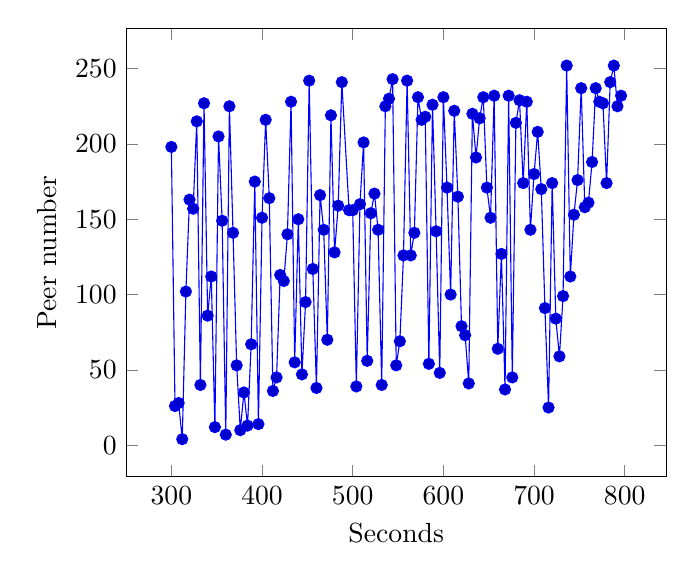
\begin{tikzpicture}
	\begin{axis}[
		xlabel=Seconds,
		ylabel={Peer number}
	]
	\addplot coordinates{
		(300,198)
		(304,26)
		(308,28)
		(312,4)
		(316,102)
		(320,163)
		(324,157)
		(328,215)
		(332,40)
		(336,227)
		(340,86)
		(344,112)
		(348,12)
		(352,205)
		(356,149)
		(360,7)
		(364,225)
		(368,141)
		(372,53)
		(376,10)
		(380,35)
		(384,13)
		(388,67)
		(392,175)
		(396,14)
		(400,151)
		(404,216)
		(408,164)
		(412,36)
		(416,45)
		(420,113)
		(424,109)
		(428,140)
		(432,228)
		(436,55)
		(440,150)
		(444,47)
		(448,95)
		(452,242)
		(456,117)
		(460,38)
		(464,166)
		(468,143)
		(472,70)
		(476,219)
		(480,128)
		(484,159)
		(488,241)
		(496,156)
		(500,156)
		(504,39)
		(508,160)
		(512,201)
		(516,56)
		(520,154)
		(524,167)
		(528,143)
		(532,40)
		(536,225)
		(540,230)
		(544,243)
		(548,53)
		(552,69)
		(556,126)
		(560,242)
		(564,126)
		(568,141)
		(572,231)
		(576,216)
		(580,218)
		(584,54)
		(588,226)
		(592,142)
		(596,48)
		(600,231)
		(604,171)
		(608,100)
		(612,222)
		(616,165)
		(620,79)
		(624,73)
		(628,41)
		(632,220)
		(636,191)
		(640,217)
		(644,231)
		(648,171)
		(652,151)
		(656,232)
		(660,64)
		(664,127)
		(668,37)
		(672,232)
		(676,45)
		(680,214)
		(684,229)
		(688,174)
		(692,228)
		(696,143)
		(700,180)
		(704,208)
		(708,170)
		(712,91)
		(716,25)
		(720,174)
		(724,84)
		(728,59)
		(732,99)
		(736,252)
		(740,112)
		(744,153)
		(748,176)
		(752,237)
		(756,158)
		(760,161)
		(764,188)
		(768,237)
		(772,228)
		(776,227)
		(780,174)
		(784,241)
		(788,252)
		(792,225)
		(796,232)
	};
	\end{axis}
\end{tikzpicture}

\end{document}